%\documentclass[acmsmall]{acmart}
% \documentclass[manuscript,screen]{acmart}
\documentclass[manuscript]{acmart}
%\documentclass[sigconf]{acmart}
%\pagenumbering{gobble}
% Rights management information. 
% This information is sent to you when you complete the rights form.
% These commands have SAMPLE values in them; it is your responsibility as an author to replace
% the commands and values with those provided to you when you complete the rights form.
%
% These commands are for a PROCEEDINGS abstract or paper.
% \copyrightyear{2021}
% \acmYear{2021}
% \setcopyright{acmlicensed}
% \acmConference[CSCW '19]{CSCW '19: ACM Conference on Computer-Supported Cooperative Work and Social Computing}{November 09--13, 2018}{Austin, TX}
% \acmBooktitle{CSCW '19: ACM Conference on Computer-Supported Cooperative Work and Social Computing, November 09--13, 2018, Austin, TX}
% \acmPrice{15.00}
% \acmDOI{10.1145/1122445.1122456}
% \acmISBN{978-1-4503-9999-9/18/06}

%
% These commands are for a JOURNAL article.
%\setcopyright{acmcopyright}
%\acmJournal{TOG}
%\acmYear{2018}\acmVolume{37}\acmNumber{4}\acmArticle{111}\acmMonth{8}
%\acmDOI{10.1145/1122445.1122456}

%
% Submission ID. 
% Use this when submitting an article to a sponsored event. You'll receive a unique submission ID from the organizers
% of the event, and this ID should be used as the parameter to this command.
%\acmSubmissionID{123-A56-BU3}

%
% The majority of ACM publications use numbered citations and references. If you are preparing content for an event
% sponsored by ACM SIGGRAPH, you must use the "author year" style of citations and references. Uncommenting
% the next command will enable that style.
%\citestyle{acmauthoryear}
% \usepackage{subfigure}

\usepackage{subcaption}
\setcopyright{rightsretained}

\copyrightyear{2021} 
\acmYear{2021} 
% \setcopyright{rightsretained} 
\acmConference[COMPASS '21]{ACM SIGCAS Conference on Computing and Sustainable Societies (COMPASS)}{June 28-July 2, 2021}{Virtual Event, Australia}
\acmBooktitle{ACM SIGCAS Conference on Computing and Sustainable Societies (COMPASS) (COMPASS '21), June 28-July 2, 2021, Virtual Event, Australia}\acmDOI{10.1145/3460112.3471981}
\acmISBN{978-1-4503-8453-7/21/06}

\begin{document}

\title{Demo: A WhatsApp Bot for Citizen Journalism in Rural India}


% The "author" command and its associated commands are used to define the authors and their affiliations.
% Of note is the shared affiliation of the first two authors, and the "authornote" and "authornotemark" commands
% used to denote shared contribution to the research.

\author{Priyanka Verma}
\affiliation{%
    \institution{Birla Institute of Technology and Science (BITS), Pilani}
    \city{Pilani}
    \state{Rajasthan}
    \country{India}
}
\email{vpriyanka0492@gmail.com}
% \orcid{1234-5678-9012}

\author{Ananya Saxena}
\affiliation{
\institution{IIIT-Naya Raipur}
\country{India}
}
\author{Alok Sharma}\affiliation{
\institution{DN Developers}
\country{India}
}
\author{William Thies}
\affiliation{
\institution{Microsoft Research}
\country{India}
}
\author{Devansh Mehta}
\affiliation{ 
\institution{Voicedeck Technologies}
\country{India}
}

% \authornotemark[1]
% \email{webmaster@marysville-ohio.com}


%
% By default, the full list of authors will be used in the page headers. Often, this list is too long, and will overlap
% other information printed in the page headers. This command allows the author to define a more concise list
% of authors' names for this purpose.
%\renewcommand{\shortauthors}{Trovato and Tobin, et al.}

%
% The abstract is a short summary of the work to be presented in the article.
\begin{abstract}
Increasing penetration of Internet-enabled smartphones in low-resource areas makes them an attractive platform for engaging emerging users. In this paper, we demonstrate how a voice forum for citizen journalism in rural India-- previously accessible via an Interactive Voice Response (IVR) system-- can be naturally supported and enriched using a chatbot. Implemented using the WhatsApp Business API, the bot enables submission of both audio (with or without image) and video stories. Following review by moderators, stories are published on a website and social media sites, and can also be browsed interactively using the WhatsApp bot. This multi-way, intermediated model of communication expands the scope and functionality of typical WhatsApp groups while offering significant cost savings relative to IVR systems. In the first 9 weeks of a long-term deployment, the bot demonstrated high usability and acceptance and resulted in 218 published stories from 27 users.
\end{abstract}

%
% Keywords. The author(s) should pick words that accurately describe the work being
% presented. Separate the keywords with commas.
\keywords{Citizen Journalism, WhatsApp, Chat bot, Low-literate users}

%
% The code below is generated by the tool at http://dl.acm.org/ccs.cfm.
% Please copy and paste the code instead of the example below.
%
\begin{CCSXML}
<ccs2012>
   <concept>
       <concept_id>10003120.10003123.10010860.10010859</concept_id>
       <concept_desc>Human-centered computing~User centered design</concept_desc>
       <concept_significance>500</concept_significance>
       </concept>
   <concept>
       <concept_id>10003120.10003138.10003140</concept_id>
       <concept_desc>Human-centered computing~Ubiquitous and mobile computing systems and tools</concept_desc>
       <concept_significance>300</concept_significance>
       </concept>
   <concept>
       <concept_id>10003120.10003138.10003141.10010895</concept_id>
       <concept_desc>Human-centered computing~Smartphones</concept_desc>
       <concept_significance>100</concept_significance>
       </concept>
   <concept>
       <concept_id>10010520.10010521.10010542.10011714</concept_id>
       <concept_desc>Computer systems organization~Special purpose systems</concept_desc>
       <concept_significance>300</concept_significance>
       </concept>
   <concept>
       <concept_id>10003120.10011738.10011776</concept_id>
       <concept_desc>Human-centered computing~Accessibility systems and tools</concept_desc>
       <concept_significance>500</concept_significance>
       </concept>
   <concept>
       <concept_id>10003120.10011738.10011775</concept_id>
       <concept_desc>Human-centered computing~Accessibility technologies</concept_desc>
       <concept_significance>500</concept_significance>
       </concept>
   <concept>
       <concept_id>10010405.10010406.10010421</concept_id>
       <concept_desc>Applied computing~Service-oriented architectures</concept_desc>
       <concept_significance>100</concept_significance>
       </concept>
 </ccs2012>
\end{CCSXML}

\ccsdesc[500]{Human-centered computing~User centered design}
\ccsdesc[300]{Human-centered computing~Ubiquitous and mobile computing systems and tools}
\ccsdesc[100]{Human-centered computing~Smartphones}
\ccsdesc[300]{Computer systems organization~Special purpose systems}
\ccsdesc[500]{Human-centered computing~Accessibility systems and tools}
\ccsdesc[500]{Human-centered computing~Accessibility technologies}
\ccsdesc[100]{Applied computing~Service-oriented architectures}







% This command processes the author and affiliation and title information and builds
% the first part of the formatted document.
\maketitle
\section{Introduction}

Online communication platforms and the mushrooming of citizen journalists have fundamentally changed our world, from Facebook groups that helped organize mass protests in Tunisia and Egypt to YouTube videos of citizens under fire from government forces in Syria. These changes have rendered an operational shift in the journalist's duty of keeping the public informed, from being a gatekeeper of information to a custodian of information who must curate, verify and lend credibility and context to content already in the public domain. Bruns~\cite{bruns_2008_active} highlights the role of journalists as shifting from “gatekeeping” to “gatewatching”, while Dailey and Starbird express the changing role of journalists by describing them as crowdsourcerers~\cite{starbird_2014_journalists} who ‘incorporate the crowd as co-collaborators’ to ‘collect, curate, synthesise, and re-broadcast information across technological divides.’

At the same time, this democratization of the information space is occuring unevenly across the world, due to varying levels of technical proficiency, infrastructural barriers and high literacy requirements for producing content on most social media platforms. Nonetheless, the smartphone revolution and its increasing penetration among the next billion users of the internet are increasing the reach of citizen journalism platforms. The intuitive interfaces on apps like Tik Tok, YouTube and WhatsApp have allowed even semi-literate users to make extensive use of these platforms, thus opening up a new design space for letting these communities become citizen journalists who can tell their own stories.

In this paper, we showcase a demo built for CGNet Swara, a citizen journalism platform based out of Central India. For over a decade, CGNet has operated an interactive voice response (IVR) platform that allows users to report or listen to stories by simply calling a toll-free number. Upon seeing that many users now have WhatsApp, we integrated their IVR number with the WhatsApp Business API, thus allowing user generated content submitted via WhatsApp to be posted on YouTube, Facebook, Twitter and CGNet's website, similar to how it is done with their IVR channel. The WhatsApp channel has been designed to supplement and not substitute for IVR, which remains an important medium for engaging communities too poor to own a smartphone, too low literate to navigate a visual interface or too remote to access the internet \cite{vashistha2019social}. We hope to contribute to the research community by both sharing our demo and the challenges we faced in designing with the WhatsApp API, and stimulating conversations around how low-resource communities can join the citizen journalism movement and share their stories with the world.


%In recent times, there has been a disruption in traditional models of journalism with the rise of information and communication technology, mainly social media platforms. The emerging paradigm of journalism- citizen journalism~\cite{gillmor_2006_we}, includes citizens as producers as well as consumers of information. Starbird expressed the changing role of journalists as crowdsourcerers~\cite{starbird_2014_journalists}, to ‘incorporate the crowd as co-collaborators’ to ‘collect, curate, synthesise, and re-broadcast information across technological divides’. Similarly, Bruns~\cite{bruns_2008_active} highlights the role of journalists to be shifting from “gatekeeping” to “gatewatching”, which requires harnessing the collective intelligence and knowledge of dedicated communities and not in ownership or control of information.

%However, not all individuals in the social pyramid have access to mainstream media outlets or social media due to technical proficiency, infrastructural and literacy barriers. However, there is now a growing number of internet users from rural India (18\% in 2019~\cite{iamai_2019_digital}) because of affordability of mobile data (Jio Effect) and rising smartphone penetration. Almost all (~99\%) rural users in India access the internet from their mobile devices and activities like social networking/chat apps and entertainment contribute to most (~80\%) of their usage of the internet~\cite{iamai_2019_digital}. Smartphones and mobile internet offer a futuristic scope for disseminating information, unlike telecenters, information kiosks based interventions, which have not proven very successful in the past~\cite{toyama_2018_from}. Hence, mobile apps like WhatsApp, YouTube open up an opportunity to act as bridge technologies to enable the rural population to contribute to citizen journalism. WhatsApp alone has 400 million users in India~\cite{iamai_2019_digital}.

%Hence, we tap the opportunity to democratise media at the grass-roots level using a chat like friendly interface. We deployed a first-of-its-kind citizen journalism platform using the WhatsApp Business API, which helps take local voices to the global level  by posting user generated content submitted via WhatsApp on YouTube, Facebook, Twitter and the organization's website. Through the technical intervention, we enable smartphone owners to access, report, and share citizen journalism reports with others. It also aids in the financial sustainability (i.e., by avoiding call costs) of the organisation. We contribute to the research community by sharing our design ideas, deployment challenges, and enabling low-resource communities to share their stories easily with global outreach for their stories.

\section{Design}
We created the chatbot for CGNet Swara, a citizen journalism platform where users give a missed call to a number, whereupon they are called back and can press `1' to report a story and `2' to hear the verified, fact-checked stories others have reported (this is cheaper than an inbound toll-free number). In the organizations 10 year history, over 100,000 unique users have called this number to report or listen, while more than 20,000 stories have been published from 6300 unique users. An internal survey found that roughly 30\% of their users had associated WhatsApp accounts, prompting our team to explore how users could submit and listen to stories through WhatsApp.

The full interaction flow of the chatbot is shown in Figure~\ref{fig:flow}. The choice for language was Hindi written in English characters. If the user sends a message other than from the WhatsApp attachments (audio, video, image, contact card and location), the bot replies with a randomly chosen story among the set of latest stories and a welcome message that includes the link to our chatbot, which can be forwarded to other users, as shown in Figure~\ref{fig:menu_contactcard_anony}. 

\begin{figure*}[htb!] 
    \centering
    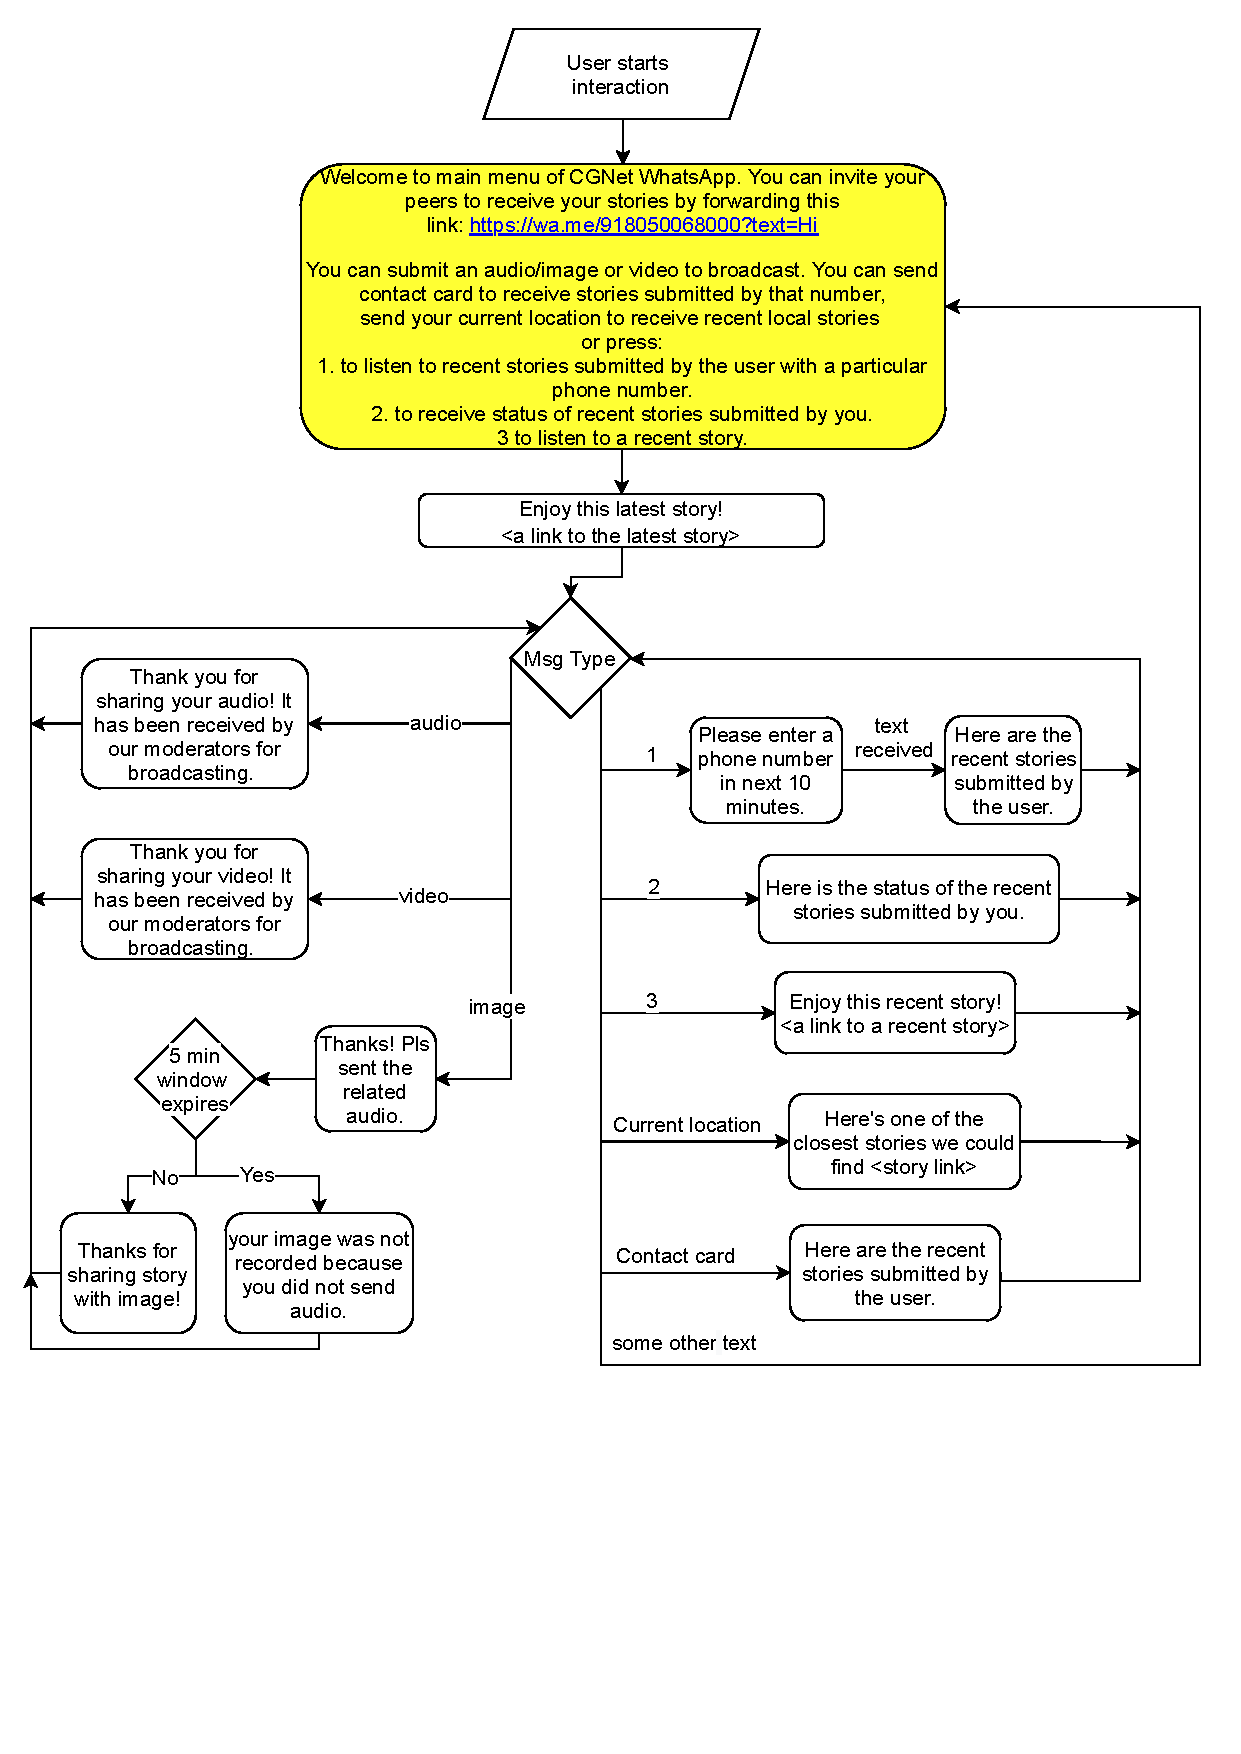
\includegraphics[width = \textwidth]{images/Final_PDF_Flow7.pdf}
    \caption{Interaction flow for content acceptance and dissemination.}
    \label{fig:flow}
    \Description[A  float image]{The image shows the interaction flow for content acceptance and dissemination through the deployed WhatsApp chat bot. The diagram begins when a user starts interaction by sending a message to the chat bot. The flow chart proceeds to display the main menu message and a link to the latest story. Then the left part of the flow chart shows that users can send audio, video or image attachments in WhatsApp to submit their stories. If a user submits image then he is asked to submit a corresponding audio story. On the right side of the flow chart, various ways of how users can request stories or status of their stories is shown. }
\end{figure*}

One of our main design constrains arose from the fact that we were designing for users who may be too low literate to navigate text content. Medhi argues that textual non-literacy is correlated with reduced cognitive skills required to navigate information architectures~\cite{medhi_2015_user}, convincing us to sacrifice greater functionality for simplicity. If a user sends a WhatsApp attachment such as an audio or video file, it is assumed to be a story submission and there is no confirmation required as users may not know how to read or type. In case more technologically proficient users want a photo to go along with their story, they can send an image, which is then followed by a request for the corresponding audio story, as shown in Figure~\ref{fig:video_image}. We tried to guide users at each step of their interaction journey through an instruction or acknowledgment based reply, although this can be tricky as users may be unable to understand these messages.

\begin{figure}[t]
    \centering
    \begin{subfigure}[b]{0.48\textwidth}
        \centering
        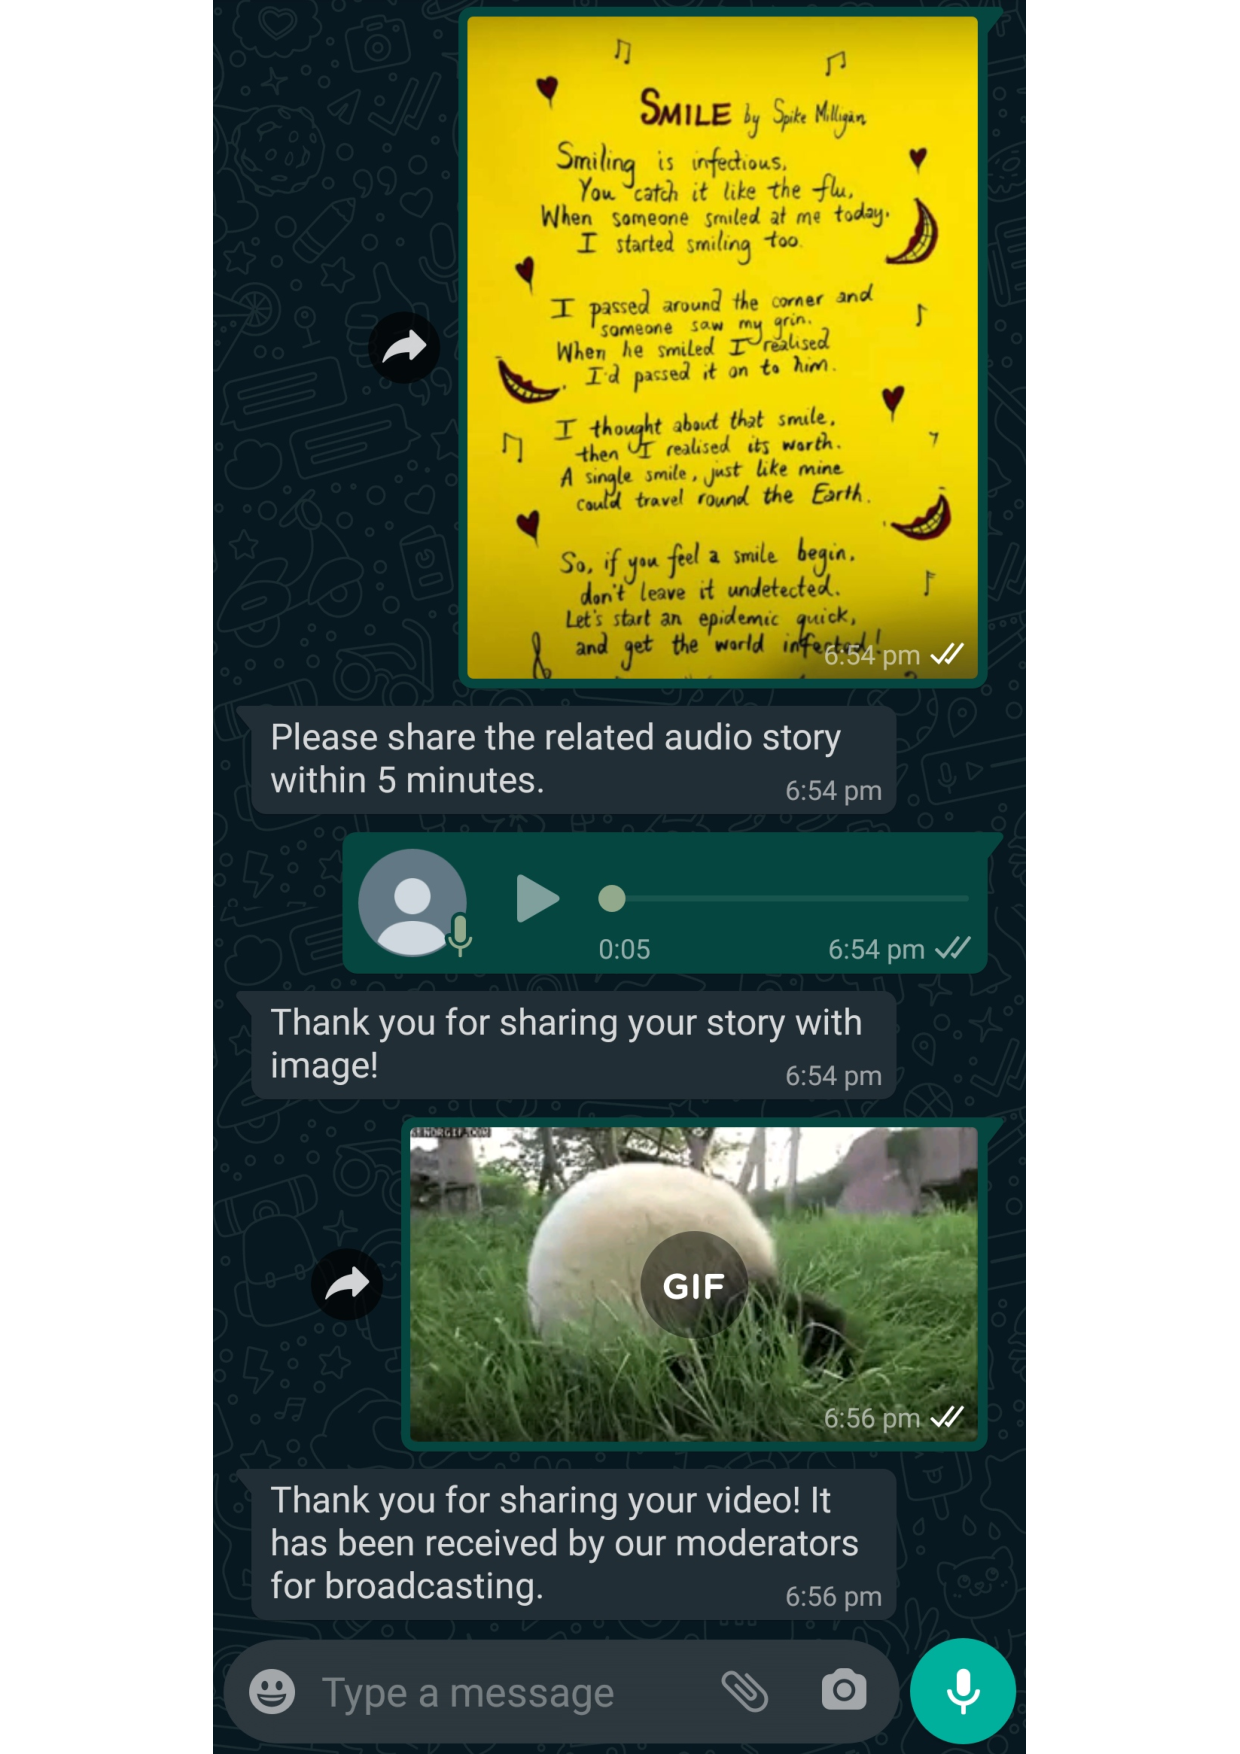
\includegraphics[height=\textwidth]{images/receive_image_video_PDF.pdf}
    \caption{Receiving video and image-based audio stories from user.}
    \label{fig:video_image}
    \end{subfigure}
    \hfill
    \begin{subfigure}[b]{0.48\textwidth}
         \centering
         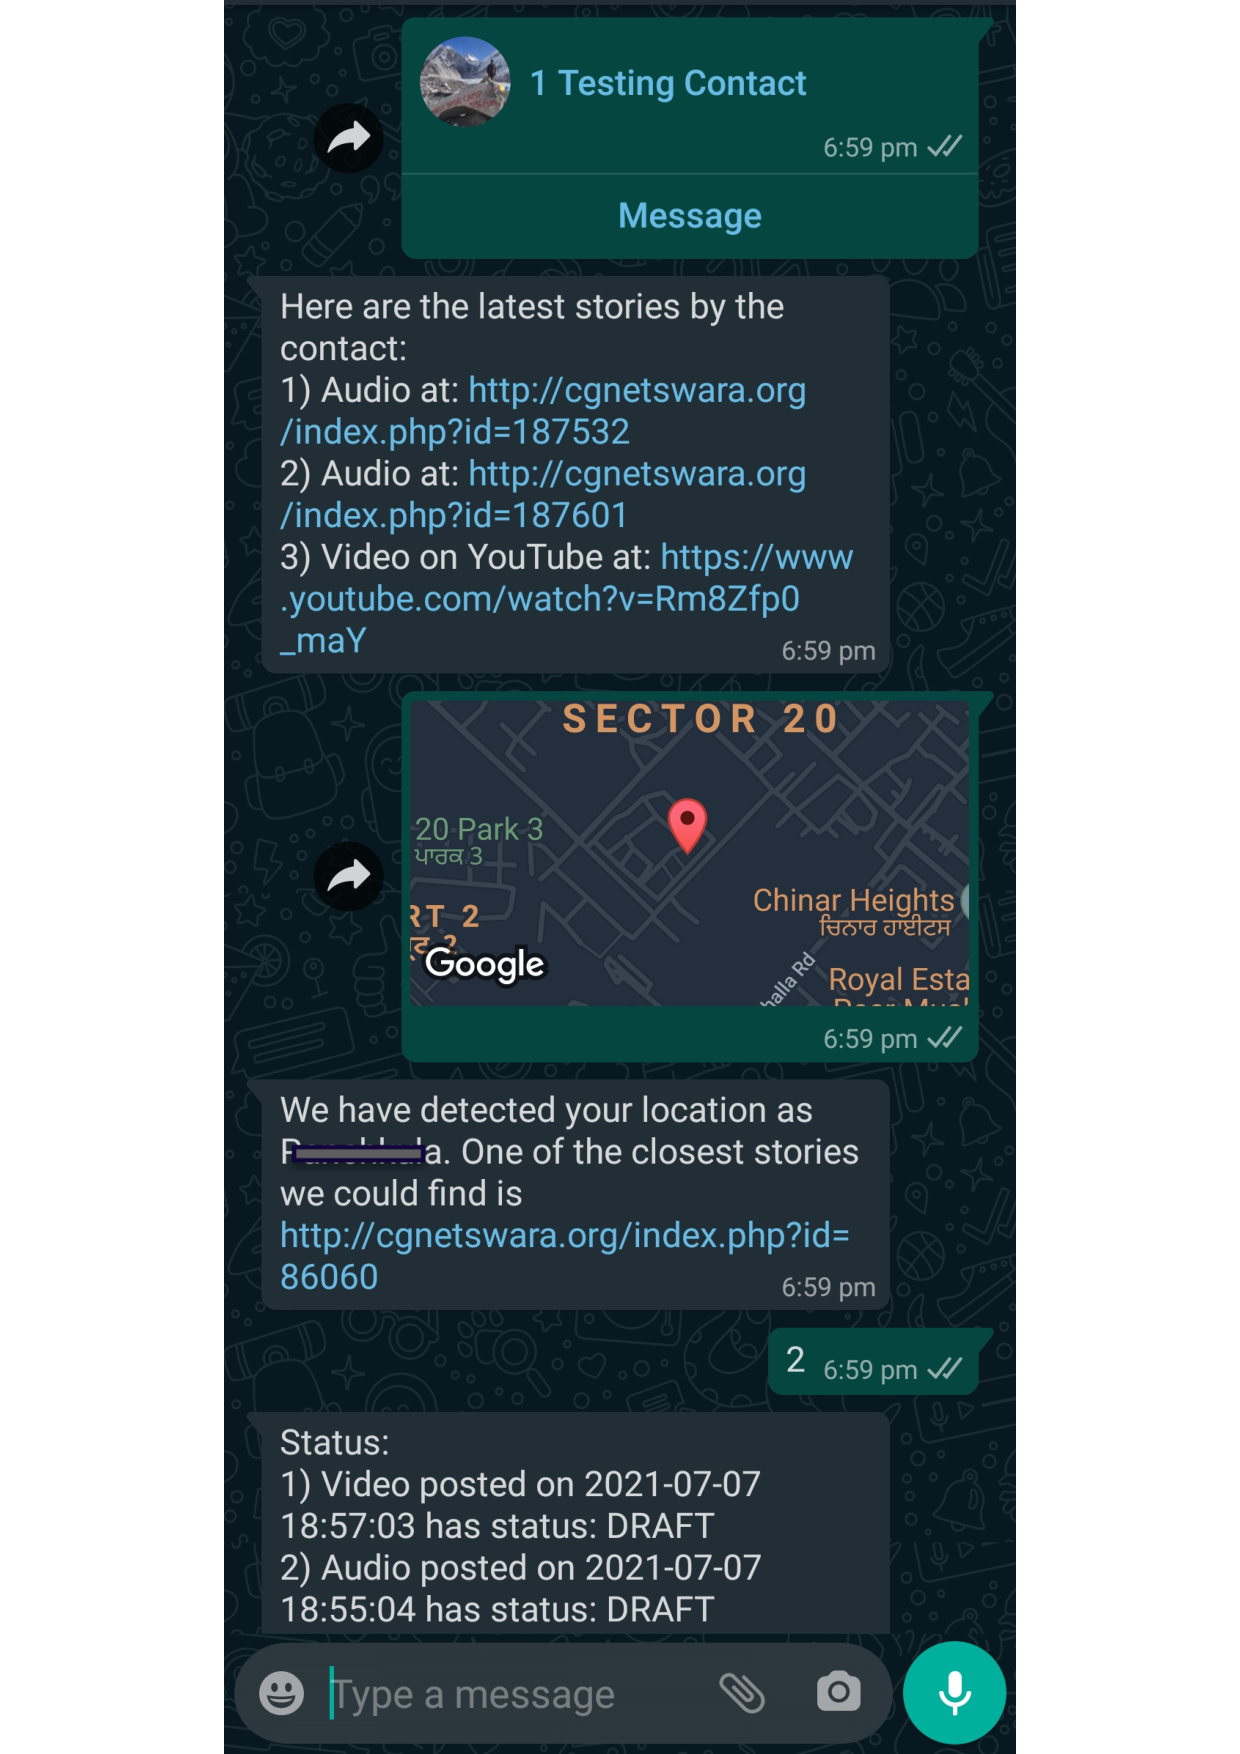
\includegraphics[height=\textwidth]{images/send_location_ccard_PDF.pdf}
    \caption{Sending latest stories and status to user.}
    \label{fig:menu_contactcard_anony}
    \end{subfigure}
    % \hfill
    % \begin{subfigure}[b]{0.31\textwidth}
    %      \centering
    %      \includegraphics[height=1.5\textwidth]{images/location.png}
    % \caption{Sending a location based story to user. Display of the features to send status of stories and the latest story.}
    % \label{fig:location}
    % \end{subfigure}
    \caption{Demo of the deployed chatbot.}
    \label{fig:two graphs}
    \Description[Two float images]{First image shows that user can send an image, followed by audio and a video to chatbot to submit his stories. The second image shows that user can send a contact card to received latest stories submitted from that phone number. It also shows that user can submit current location to receive latest local stories from that area and when user presses 2, he received the status of recent stories submitted by him.}
\end{figure}

We also designed our chat interface so that it could be operated with minimal number of steps and without any textual input. If users want to listen to more stories, they can do that by typing in `3' at anytime, without having to return to the main menu. Users may also request for stories reported by another user by typing in `1' and then entering the phone number of the person whose stories they wish to listen to, or by directly sending a contact card attachment (Figure~\ref{fig:menu_contactcard_anony}). Similarly, users can listen to stories reported by users in their district by simply sending the location attachment (through the 'Send current location' feature). Additionally, more literate users can request for the status of their unpublished stories by typing in `2'- a personalised feedback mechanism that could not only help increase their engagement but also build accountability in the organisation so that users can complain to the staff if their story has been left unattended. 

%While the IVR platform of the organisation has shown remarkable promise in reaching populations too poor to own a smartphone, too low literate to navigate text content or too remote to access the internet, they have also had difficulty in scaling up due to inefficient cost structures compared to internet platforms. A smartphone app has been deployed to provide more functionality to users than IVR like sharing audios, saving media on phone storage, however, there are additional overheads of installation and training. On the contrary, WhatsApp is one of the most used social media platforms in rural India~\cite{statista_2018_social, tandon_2016_rural}. The WhatsApp channel has been thus designed as a supplement to and not a substitute of IVR or smartphone app. 

A second set of design constraints came from our team having to integrate as far as possible with the existing workflow used by CGNet. For example, editing and reviewing stories submitted via IVR takes place on the open-source loudblog moderation platform, forcing us to modify its capabilities to accept video submissions made over WhatsApp. A regular account on WhatsApp would not have allowed us to take audio or video submissions directly onto the moderation platform, prompting us to explore the API which comes with a fixed cost of USD 500 per month and has its own set of design constraints. WhatsApp bots can reply for free within a 24 hour window from the user's last message, while initiating a conversation outside this window incurs marginal costs of USD 0.005 per message and also requires both permission from the user and that the message be pre-approved by Facebook. To minimize cost and complexity, we designed the bot such that it only replies to users.
% 
% or those from another user by sharing their contact card.

% \begin{figure}
%     \centering
%     \includegraphics[height= 0.7\textwidth]{images/video_image_dark.png}
%     \caption{Receiving video and image based audio stories from user.}
%     \label{fig:video_image_dark}
% \end{figure}

% \begin{figure}
%     \centering
%     \includegraphics[height= 0.8\textwidth]{images/video_image.jpg}
%     \caption{Receiving video and image based audio stories from user.}
%     \label{fig:video_image}
% \end{figure} 

%Similarly, instead of asking users to optionally submit an image associated with an audio story, the bot asks for a compulsory corresponding audio when a user submits an image. The former method would add one more level of depth as it would require users to input an additional message to confirm if an audio submitted after an image is associated with it, therefore was rejected to reduce cognitive load of users. . For the same reason, users are not asked to press a button to confirm their submission, unlike in the case of IVRs.    

The third and final set of factors influencing our design was the needs and capacities of CGNet Swara. To save space and reduce load on their IVR server, videos are hosted on YouTube and dissemination of stories on WhatsApp is done through sending links instead of the actual media file. Audio is automatically extracted from videos received via WhatsApp, so that they can be separately edited and played over the IVR channel. We also found that many of the staff reporters earlier faced issues with space on their phone for storing video or audio interviews they took while in the field, which was mitigated by having them simply send those media files to the WhatsApp chatbot we designed.

In the future, we have plans to introduce a special ``moderator mode'' on the WhatsApp bot that would reduce the workload of editors on the moderation platform. Experienced reporters in the field would be able to type in metadata about the story they are reporting, such as its title and description, which are currently filled in by moderators.

%Users not owning a smartphone, can have their story reported by reporters on field visits, who can access a special 'Moderator' mode. This feature specifically helps to distinguish between the reporter and owner of the story, i.e, through this feature the owner of story can be identified even if his/her story has been submitted by a reported. Additionally, reporters can type in metadata, such as its title and description to reduce the work of the backend moderation team. This metadata could then be manually typed in the loudblog website. 


%To save space on and distribute load from the server, YouTube is chosen over the organisation's front facing website for hosting final videos, and to leverage other advantages like global outreach, richer viewer analytics and monetizability. Due to internet constraints of users in rural areas, the dissemination of stories was done by sending links to media hosted on YouTube or on the organisation website, instead of actual media file.



% \begin{figure}
%     \centering
%     \includegraphics[width= 0.8\textwidth]{images/phone_stories.png}
%     \caption{Sending users stories submitted by the contact number typed by them.}
%     \label{fig:send_phone_story}
% \end{figure}

% \begin{figure}
%     \centering
%     \includegraphics[width=0.8 \textwidth]{images/status_stories.png}
%     \caption{Sending users the status of the latest stories submitted by them. Like other features, users can access this feature after the main menu or at any other stage of the interaction flow.}
%     \label{fig:send_status}
% \end{figure}

% 
\section{Deployment}

In 28 days of deployment, a total of 236 stories were reported by 25 unique users, of which 126 have been fact-checked, verified and published online (Table~\ref{tab:usage_data}). Only 2 video stories have been published out of 37 submissions, due in part to the CGNet moderators lacking video editing skills. One of the videos was sent by an old man who sang a song,

\textit{``You would see that we will defeat Corona. We will not participate in mass gathering. You would see that we will defeat Corona. We will not hug or shake hands with each other...''
}
%As seen in Table~\ref{tab:usage_data}, 

The majority of stories comprise accounts of violence inflicted by insurgent or government forces (CGNet operates in a region experiencing more than 30 years of civil war). This may be due to CGNet preferring to first test the chatbot with their own reporters, who are tasked with reporting stories of victims caught in the conflict, before publicizing it to other citizen journalists who currently use their IVR channel as a cultural repository and to report longstanding community issues. The chatbot nevertheless received 45 stories centered around basic governance problems that show how citizen journalists can speak truth to power. For example, despite government claims of electrifying all villages in India, we received the following report from a user in the Central Southern state of Telangana;

\textit{``Since past 15 years, the villagers are facing electricity problems due to which we do not have proper lighting facility here. We have to stay in dark during night times due to lack of electricity. Advanced facilities are also not available. I appeal to you all for help.''
}

Only 2 impact stories were recorded where users updated us that the problem they reported earlier had been resolved. Future work will need to look more carefully at developing mechanisms to solve issues raised on the platform.

%Our WhatsApp based citizen journalism platform has been live for 28 days at the time of writing. The usage numbers  after 28 days of deployment are shown in . The organisation has not publicized the presence of their WhatsApp channel, preferring to first test it with their own staff reporters.

\begin{table}[!htbp]
    \centering
    \caption{Usage data for 9 weeks of deployment.}
    \begin{tabular}{l l}
        \noalign{\smallskip}\midrule
        Parameter & Count \\
        \noalign{\smallskip}\midrule
        Total stories received via WhatsApp &	539  \\
        Stories published on web & 218	 \\
        Distinct users	& 27 \\
        Total video stories received & 93	\\
        Video stories published & 4	\\
        \noalign{\smallskip}\hline
    \end{tabular}
    
    \label{tab:usage_data}
\end{table} 


% \begin{table}[!htbp]
%     \centering
%     \caption{Classification of Stories}
%     \label{tab:classification}
%     \begin{tabular}{c c}
%         \noalign{\smallskip}\hline
%         Story Type & Count  \\
%         \hline\noalign{\smallskip}
%         Victim &	78 (62\%) \\
%         Problems & 45 (36\%)	 \\
%         Impact	& 2 (2\%)\\
%         Song & 1 (<1\%)	\\
%         \noalign{\smallskip}\hline
%     \end{tabular}
% \end{table} 


%\begin{table}[h]
%\caption{Analysis of stories submitted via WhatsApp which have been published online.}
%    \begin{subtable}[h]{0.49\textwidth}
%    \centering
%    \caption {Classification of stories.}
%    \begin{tabular}{l l}
%        \noalign{\smallskip}\midrule
%        Story Type & Count   \\
%        \noalign{\smallskip}\midrule
%        Victim &	117 (53.67\%) \\
%        Problems & 81 (37.16\%)	 \\
%        Song & 8 (3.67\%)	\\
%        Impact	& 6 (2.76\%)\\
%        For Awareness & 4 (1.84\%) \\
%        Story & 2 (<1\%)	\\
%        \noalign{\smallskip}\bottomrule
%    \end{tabular}
%    \label{tab:classification_stories}
%    \end{subtable}
%    \hfill
%    \begin{subtable}[h]{0.49\textwidth}
%    \centering
%     \caption {Classification of problem stories.}
%    \begin{tabular}{l l }
%         \noalign{\smallskip}\midrule
%         Problem Type  & Count \\
%        \noalign{\smallskip}\midrule
%        Water  & 35 (43.21\%)  \\
%        Ration card  & 8 (9.88\%)	\\
%        Road & 13 (16.05\%)  \\
%        Electricity & 4 (4.94\%) \\
%        Pension & 11 (13.58\%) \\
%        Miscellaneous & 10 (12.34\%) \\
%        \noalign{\smallskip}\bottomrule
%    \end{tabular}
%   
%    \label{tab:classification_problem}
%    \end{subtable}
%    \label{fig:smartphone_features}
%    
%\end{table}

\begin{table}[h]
\caption{Analysis of stories submitted via WhatsApp which have been published online.}
\centering

\begin{tabular}{@{}c@{}}
    %\begin{subtable}[h]{0.49\textwidth}
\multicolumn{1}{@{}c@{}}{\bf (a) Classification of stories.}\\ \hline
    
    %\caption {Classification of stories.}
\tabcolsep12pt
    \begin{tabular}{l l}\hline
        
        Story Type & Count   \\ \hline
        
        Victim &	117 (53.67\%) \\
        Problems & 81 (37.16\%)	 \\
        Song & 8 (3.67\%)	\\
        Impact	& 6 (2.76\%)\\
        For Awareness & 4 (1.84\%) \\
        Story & 2 (<1\%)	\\
        \hline
    \end{tabular} \\\\
    %\label{tab:classification_stories}
    %\end{subtable}
\multicolumn{1}{@{}c@{}}{\bf (b) Classification of problem stories.}\\ \hline
    %\begin{subtable}[h]{0.49\textwidth}
    %\centering
     %\caption {Classification of problem stories.}
\tabcolsep13pt
    \begin{tabular}{l l }
         \hline
         Problem Type  & Count \\
        \hline
        Water  & 35 (43.21\%)  \\
        Ration card  & 8 (9.88\%)	\\
        Road & 13 (16.05\%)  \\
        Electricity & 4 (4.94\%) \\
        Pension & 11 (13.58\%) \\
        Miscellaneous & 10 (12.34\%) \\
        \hline
    \end{tabular}
   \end{tabular}

    %\label{tab:classification_problem}
    %\end{subtable}
    \label{fig:smartphone_features}
    
\end{table}
\section{Discussion}

The use of WhatsApp in India has been transcending class boundaries~\cite{mint_2018_how}, motivating us to explore whether its API can be used for distributing and crowdsourcing stories from communities that may not even be able to read or write. Our demo enabled users to contribute content in video, voice and vernacular- 3Vs that have been central to the growth of Internet users in India~\cite{google_2020_3V}. In particular, augmenting the phone numbers of existing IVR platforms with the WhatsApp API to allow users to submit videos (as opposed to only audio) has immense potential in scaling up the voices of marginalized communities and promoting linguistic diversity to create a more inclusive Internet. However, this model relies upon an ecosystem of cheap  mobile data, since users use their own bandwidth for submissions via WhatsApp unlike an IVR platform that relies upon a simple missed call.

Another community media platform making extensive use of WhatsApp is Khabar Lahariya~\cite{sinha_2018_reimagining}, whose reporters use WhatsApp to send videos to a central editorial team for processing and dissemination across multiple platforms and news organizations. We would argue that use of the WhatsApp API, which allows for providing acknowledgements, explanations, instructions and updates through automatic replies, is more accessible to people at the grassroots who want to be journalists and report their own stories. Compared to using a regular WhatsApp account for receiving stories, the API allows for a more robust two-way communication with grassroots communities that can be used to distribute stories back to them and conduct short polls, surveys and interviews. At the same time, expanding the base of reporters requires clear disclosure policies, as many may not be aware that stories they report are uploaded with their name against it and will remain on the internet for posterity.

Finally, an emerging body of research speaks to the benefit of `meeting people where they are' or integrating with existing platforms already in use, rather than creating unfamiliar, custom-built platform \cite{lambton2020unplatformed, saldivar2019online}. CGNet's earlier attempts to crowdsource and distribute stories through dedicated smartphone applications floundered due to the training and installation overheads for onboarding new users \cite{d2014mobile, mehta2020facilitating}. By contrast, the CGNet field team now simply instructs new users to call the IVR number and report their stories if they do not have internet, or to WhatsApp them to the same number if they have a smartphone. If there is one takeaway we hope researchers and practitioners will absorb from this short paper, it is this: why build an app, when you can use WhatsApp?

% \section{Acknowledgements}

% We would like to thank Aditya Vashistha and Amit Sharma for their comments on an early outline of this paper and Shubhranshu Choudhary at CGNet Swara for his participation in the design process. We are also grateful to the Center for Societal Impact through Cloud and AI (SCAI) at Microsoft Research India for their steadfast support over the years.

%Through this demo, we demonstrate how IVR based platforms can evolve as more and more people get access to the internet and smartphones. . This solution is one step above earlier efforts as WhatsApp offers richer media over the traditional IVR system, which is also challenging to scale due to cost; no training/installation is required, unlike in other smartphone apps based interventions. WhatsApp also caters to users with intermittent internet access, as users can report stories without the Internet which then get submitted whenever they get to access the internet. 
% Both of these extensions are truly empowering for emerging users, who have limited familiarity with interfaces such as IVR and special-purpose apps, but are increasingly familiar and comfortable with WhatsApp.


 %In contrast the organisation X trains and enables people to do their own reporting. While the organisation X has to pay the fixed cost of $\$500$ per month for hosting the WhatsApp Business API, it has its advantages of offering a friendly chat-like feeling to users through . Apart from its use for citizen journalism, the WhatsApp channel can be further used to conduct short polls, surveys, interviews for collecting grass-root level data. It would be of interest to replicate studies like Learn2Earn~\cite{swaminathan_2019_learn2earn} by leveraging the richer media content.


%In future, the dissemination of stories can be improved by developing personalised recommendation system. The organisation also plans to customise the user experience by providing the functionality to enable users to request locally relevant stories by asking them to share their location via the `Share current location' feature of WhatsApp. Another design feature in development is- `Moderator Mode', for provision of differentiating the stories submitted by users from stories submitted by reporter for a rural user without a smartphone. This mode would be beneficial for the organisation to keep track of and design incentive schemes based on progress of reporters, e.g., stories submitted by a moderator per day, and for the on-field moderators/reporters, e.g., they can type in metadata, such as its title and description to reduce the work of the backend moderation team.

% While the main purpose of the 'Moderator Mode' has been to differentiate the stories submitted by users from stories submitted by moderators for someone else, in future, the backend program for this mode can be programmed to automatically upload the metadata received by moderators to the loudblog website. This mode would also be helpful for the organisation in future to keep track of progress of moderators, e.g., stories submitted by a moderator per day and design incentive schemes for them enable maximum stories submission. 
% Users not owning a smartphone, can have their story reported by reporters on field visits, who can access a special 'Moderator' mode. This feature specifically helps to distinguish between the reporter and owner of the story, i.e, through this feature the owner of story can be identified even if his/her story has been submitted by a reported. Additionally, reporters can type in metadata, such as its title and description to reduce the work of the backend moderation team. This metadata could then be manually typed in the loudblog website. 

%Users not owning a smartphone, can have their story reported by reporters on field visits, who can access a special 'Moderator' mode. This feature specifically helps to distinguish between the reporter and owner of the story, i.e, through this feature the owner of story can be identified even if his/her story has been submitted by a reported. Additionally, reporters can type in metadata, such as its title and description to reduce the work of the backend moderation team. This metadata could then be manually typed in the loudblog website. 


%growth of internet, initial software companies that built operating systems (microsoft, apple), then in the social web came companies that built on top of operating systems (amazon, google, facebook) and we now believe we are heading into the networked web where next big internet companies will build off the companies that became big in the social web, similar to how those companies built off the ones that created operating systems. can see advantages of unplatforming very clearly, no app or installation required. some countries like china are already ahead of the curve, where new businesses only opt for wechat page and dont even have their own platform or website.

%importance of having a hybrid model, if only build a platform for low network users, only those will end up using it as people with higher connectivity will migrate to those other platforms. important to evolve with a community while still ensuring no one is left behind, ahve tried to do that with hybrid where people can either call if no internet or whatsapp if they have a smartphone and connectivity. focus on just bottom of the pyramid without the layers above will pose sustainability problems among other issues.

%sustainability for the organization, ivr unable to scale while this one can. it is also limited in its functionality, unlike whatsapp.


\begin{acks}
We would like to thank Aditya Vashistha and Amit Sharma for their comments on an early outline of this paper and Shubhranshu Choudhary at CGNet Swara for his participation in the design process. We are also grateful to the Center for Societal Impact through Cloud and AI (SCAI) at Microsoft Research India for their steadfast support over the years.
\end{acks}

%\input{body}


\bibliographystyle{ACM-Reference-Format}
\bibliography{references}

\end{document}
